\documentclass{standalone}
\usepackage{tikz}
\usepackage{pgfplots}
\pgfplotsset{width=32cm,height=18cm,compat=1.3}
\pgfplotsset{every tick label/.append style={font=\Huge}}
\usepackage{filecontents}
\usepgfplotslibrary{fillbetween}

\usetikzlibrary{patterns}

\definecolor{citrine}{rgb}{0.89, 0.82, 0.04}

\begin{document}
	\centering
		\vspace{1.5em}
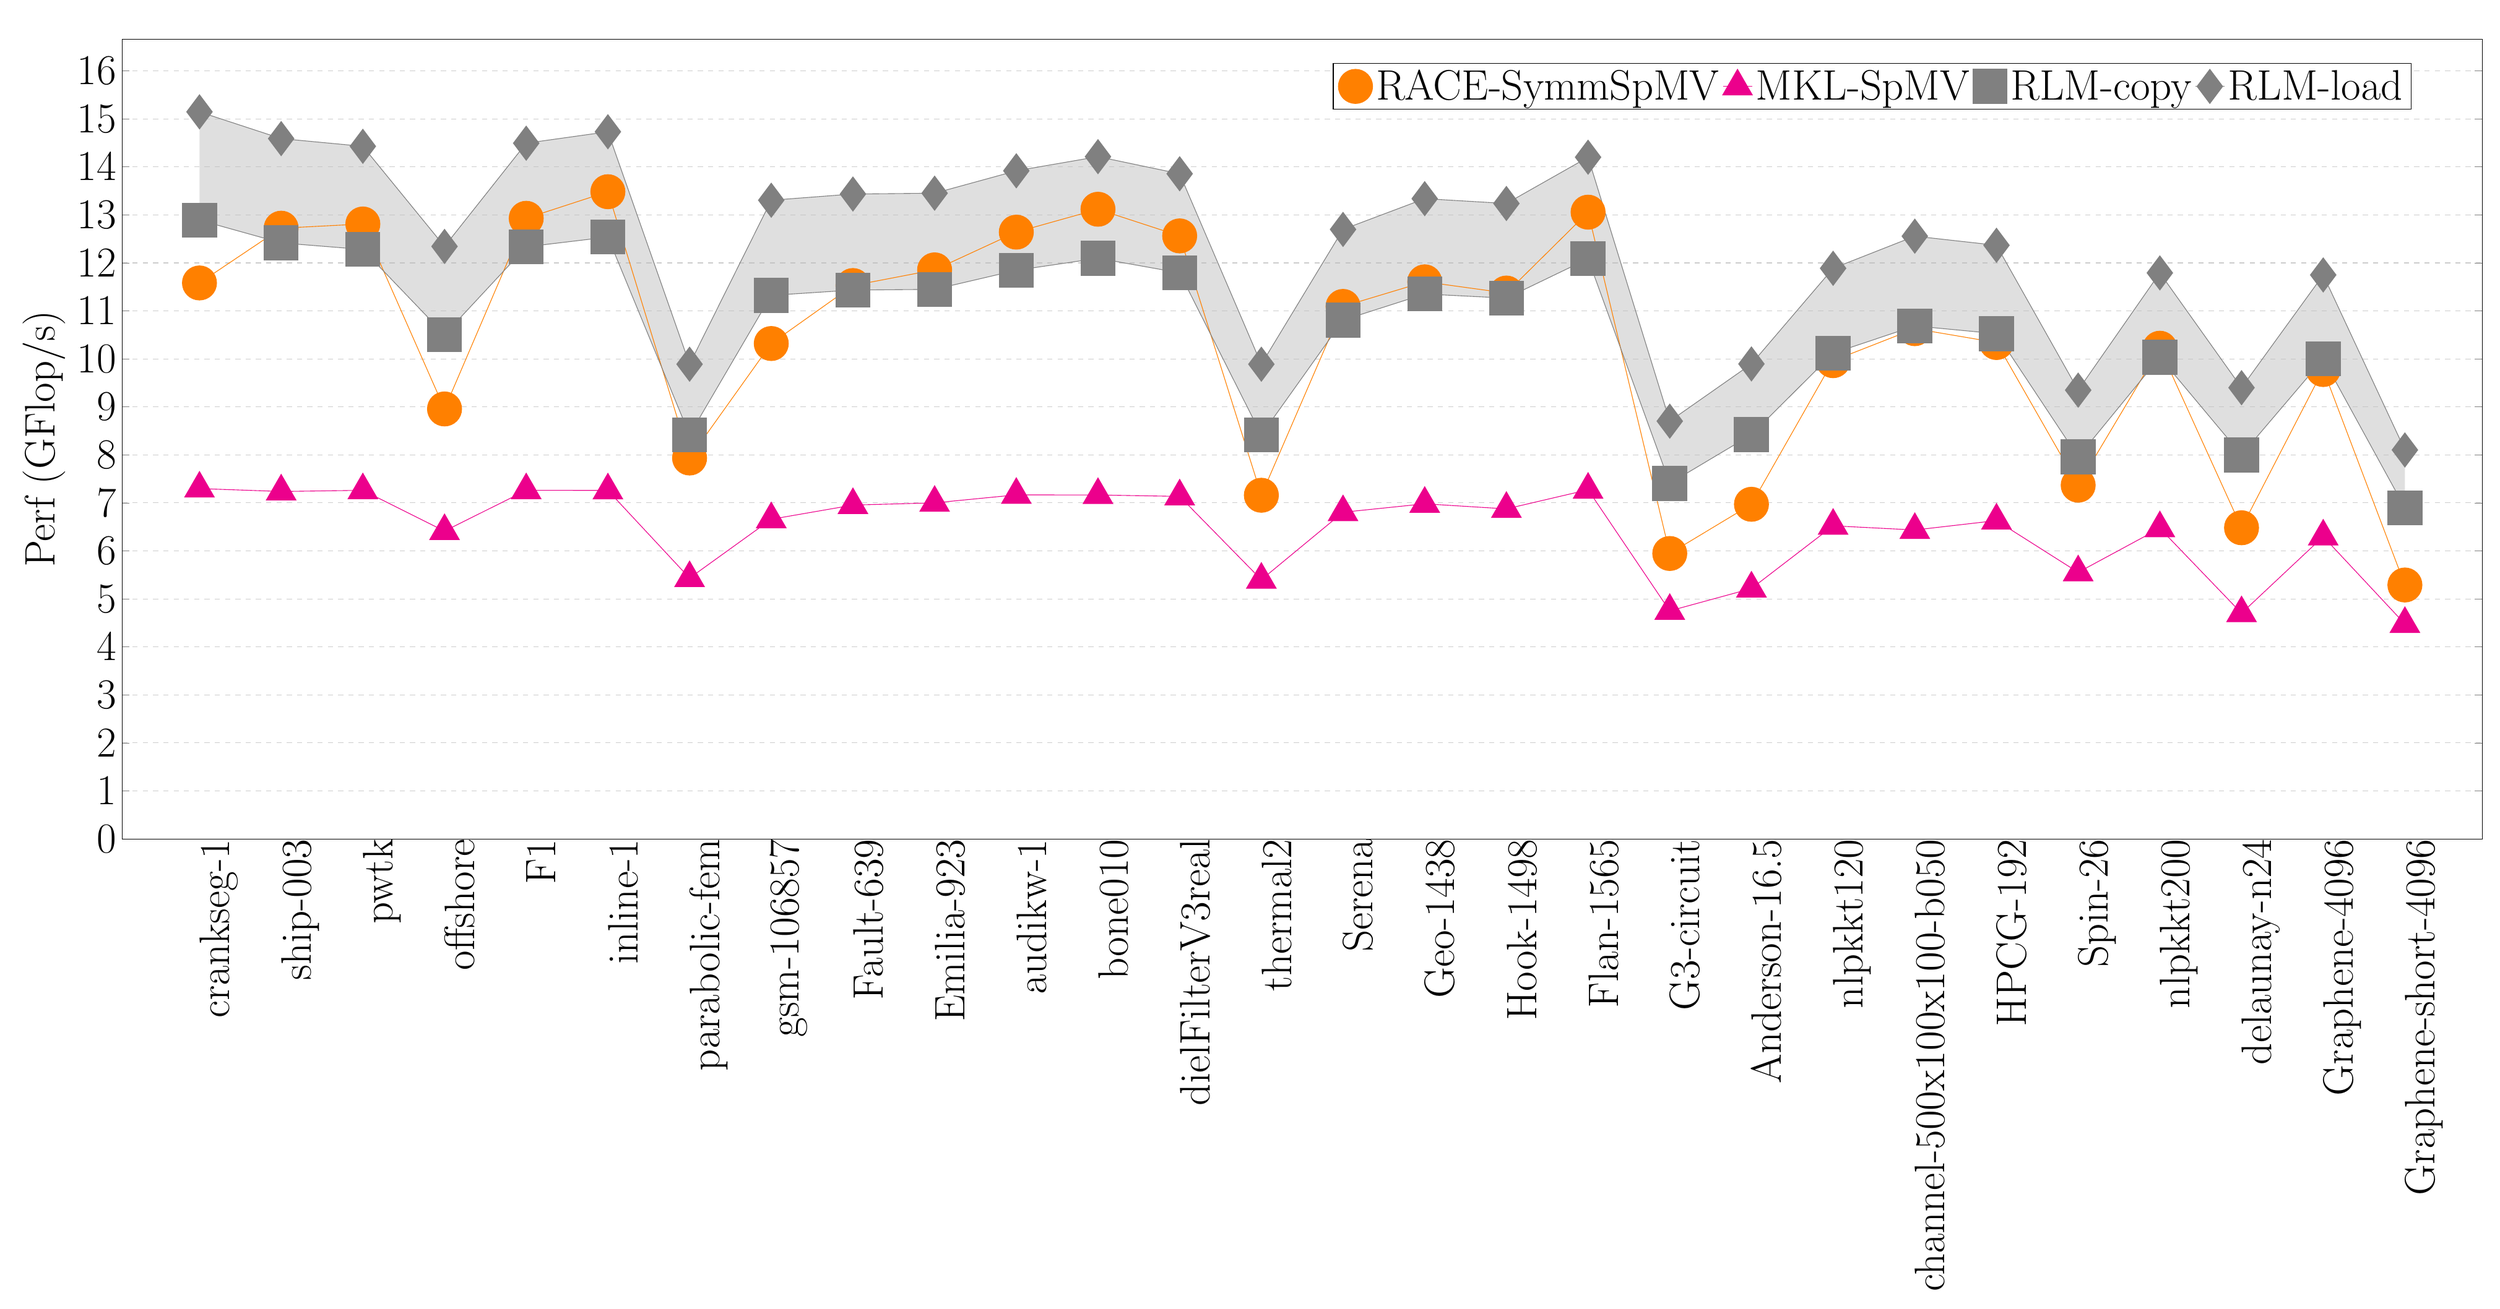
\begin{tikzpicture}
		%	\node at (13.25,15) {\LARGE{}};
			\begin{axis}[
		%	xmin=0.25, xmax=7.25,
			ymin=0, %ymax=3.25,
			xtick={1, 2, 3, 4, 5, 6, 7, 8, 9, 10, 11, 12, 13, 14, 15, 16, 17, 18, 19, 20, 21, 22, 23, 24, 25, 26, 27, 28},
		%	ytick={0,0.5,1,1.5,2,2.5,3},
			xticklabels={crankseg-1, ship-003, pwtk, offshore, F1, inline-1, parabolic-fem, gsm-106857, Fault-639, Emilia-923, audikw-1, bone010, dielFilterV3real, thermal2, Serena, Geo-1438, Hook-1498, Flan-1565, G3-circuit, Anderson-16.5, nlpkkt120, channel-500x100x100-b050, HPCG-192, Spin-26, nlpkkt200, delaunay-n24, Graphene-4096, Graphene-short-4096},
			width  = 50cm,
			height = 18cm,
			major x tick style = transparent,
			%	minor ytick={1, 5, 10, 15, 20, 25, 30 ,35,40},
			grid = minor,	
			%add_bar_commands
			ymajorgrids = true,
			grid style={dashed, gray!40},
			ylabel = {\Huge{Perf (GFlop/s)}},
		%	symbolic x coords={Graphene-2048-2048, Graphene-4096-4096, Spin-24-24-24},
			x tick label style={rotate=90, anchor=north east, inner sep=0mm, font={\Huge}},
			tick label style={font={\Huge}},
			scaled y ticks = false,
			enlarge x limits=0.035,
			legend cell align=left,
			legend style={font=\Huge},
			legend columns=-1,
			legend style={
				%at={(1,1.05)},
				%anchor=south east,
				%column sep=1ex,
				legend pos=north east
			},
			%spl_legend_code
			title= {\Huge\scalebox{1.5}{{}}}
			]

\addplot[name path=RACE-SymmSpMV, mark=*, mark size=10pt, mark options={orange}, draw=orange ] plot coordinates{(1,11.581950) (2,12.722942) (3,12.810374) (4,8.957090) (5,12.928522) (6,13.482575) (7,7.934556) (8,10.319803) (9,11.528034) (10,11.854632) (11,12.640306) (12,13.117369) (13,12.562132) (14,7.158996) (15,11.093061) (16,11.605302) (17,11.371847) (18,13.056664) (19,5.945987) (20,6.970780) (21,9.962605) (22,10.629349) (23,10.340284) (24,7.368607) (25,10.221975) (26,6.481632) (27,9.777899) (28,5.289580)};
\addplot[name path=MKL-SpMV, mark=triangle*, mark size=10pt, mark options={magenta}, draw=magenta ] plot coordinates{(1,7.297855) (2,7.237710) (3,7.261922) (4,6.412715) (5,7.261814) (6,7.259657) (7,5.433150) (8,6.658801) (9,6.954289) (10,7.000728) (11,7.166920) (12,7.164436) (13,7.135097) (14,5.399340) (15,6.805161) (16,6.980648) (17,6.874971) (18,7.273237) (19,4.750522) (20,5.215657) (21,6.522366) (22,6.435327) (23,6.631285) (24,5.552821) (25,6.471373) (26,4.701179) (27,6.298699) (28,4.477674)};
\addplot[name path=RLM-copy, mark=square*, mark size=10pt, mark options={gray}, draw=gray ] plot coordinates{(1,12.890740704234203) (2,12.416207253432326) (3,12.279716689527307) (4,10.50476953954768) (5,12.334849461214413) (6,12.537926458618394) (7,8.416496094137019) (8,11.323601760908645) (9,11.433949162013397) (10,11.448241355528609) (11,11.845401186536506) (12,12.096117795887302) (13,11.792916996257055) (14,8.415994333317869) (15,10.806105736422975) (16,11.35147027588552) (17,11.26582239667989) (18,12.086376233776319) (19,7.4065933293667285) (20,8.421052631578947) (21,10.116700898525137) (22,10.686412420028812) (23,10.524941807760008) (24,7.956377832470507) (25,10.035067367477408) (26,7.99999314286302) (27,9.999049636594167) (28,6.896035691405395)};
\addplot[name path=RLM-load, mark=diamond*, mark size=10pt, mark options={gray}, draw=gray ] plot coordinates{(1,15.146620327475189) (2,14.589043522782982) (3,14.428667110194585) (4,12.343104208968525) (5,14.493448116926935) (6,14.732063588876613) (7,9.889382910610996) (8,13.305232069067657) (9,13.434890265365741) (10,13.451683592746114) (11,13.918346394180395) (12,14.212938410167581) (13,13.856677470602039) (14,9.888793341648496) (15,12.697174240296995) (16,13.337977574165485) (17,13.23734131609887) (18,14.201492074687176) (19,8.702747162005906) (20,9.894736842105262) (21,11.887123555767037) (22,12.556534593533854) (23,12.366806624118011) (24,9.348743953152846) (25,11.791204156785955) (26,9.399991942864048) (27,11.748883322998147) (28,8.102841937401339)};
\addplot[fill=lightgray,opacity=0.5]
fill between[of= RLM-copy and RLM-load];
	%addplot cmd

	\legend{RACE-SymmSpMV, MKL-SpMV, RLM-copy, RLM-load}

	\end{axis}			
\end{tikzpicture}

\end{document}

